% !TEX root = ../main.tex
\subsection{CEBAF}
\label{11.100::cebaf}
    \begin{figure}[b!]
        \centering\frame{
        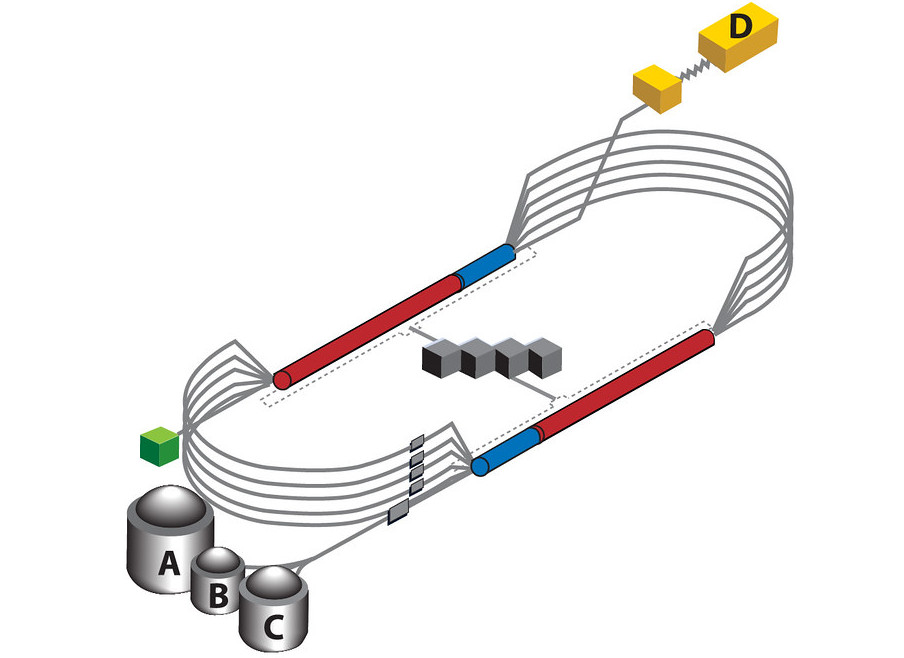
\includegraphics[width=\textwidth]{100cebaf_diagram.jpg}}
        \caption[CEBAF.]{Simplified representation of CEBAF.
        Source: \href{https://jlab.org/}{jlab.org}.}
        \label{fig::11.100::cebaf}
    \end{figure}

    The CEBAF facility consists of a pair of 1.4-km-long antiparallel superconducting radio-frequency (RF) linear accelerators (linacs) constructed 8 meters below the surface.
    The two accelerators are connected by two 180-degree arcs, each with a radius of 80 meters \cite{leemann2001}.
    A schematic diagram illustrating the design of CEBAF is provided in Figure \ref{fig::11.100::cebaf}.

    The recirculating arcs are composed of five separate beamline sections, allowing the beam to traverse each linear particle accelerator (linac) up to five times.
    Within each linac, the energy gain of the beam ranges from 0.8 GeV to 1.2 GeV, resulting in a final beam energy of approximately 12 GeV.
    CEBAF is specifically designed for high-energy electron beam experiments aimed at studying the structure of mesons, nucleons, and nuclei \cite{rode2010}.
